\section{Autonomous Equations and Population Dynamics}
    Autonomous equations are those of the form
    \begin{equation*}
        dy/dt = f(y)
    \end{equation*}
    This form of equation is separable.
    \newline
    \textbf{Exponential Growth.} Exponential growth has an equation of the form 
    \begin{equation*}
        dy/dt = ry
    \end{equation*}
    where the constant of proportionality $r$ is called the \textbf{rate of growth or decline}. Solving this with the initial condition $$y(0) = y_0$$ we obtain $$y = y_0e^{rt}$$
    For many populations this equation holds true to a certain extent but this is not sustainable since the population would grow rapidly.
    \newline
    \textbf{Logistic Growth.} Since the growth rate actually depending on the population, we replace the constant $r$ with $h(y)$. So, 
    \begin{equation*}
        dy/dt = h(y)y
    \end{equation*}
    The Verhulst equation or the \textbf{logistic equation} is of the form
    \begin{equation*}
        dy/dt = (r-ay)y
    \end{equation*}
    which is the same as the last equation with $h(y) = (r - ay)$ so that $h(y) \approx r$ when y is small and it decreases as y increases. The logistic equation if often written as 
    \begin{equation*}
        \frac{dy}{dt} = r(1 - \frac{y}{K})y
    \end{equation*}
    where $K = r/a$. $r$ is called the \textbf{intrinsic growth rate}, the growth rate in the absence of limiting factors. 
    \newline \indent
    The constant solutions, or \textbf{equilibrium solutions}, occur when
    \begin{equation*}
        \frac{dy}{dt} = r(1 - \frac{y}{K})y = 0
    \end{equation*}
    or at $y = 0$ and $y = K$. These are also called \textbf{critical points}. 
    \newline \indent
    Other solutions for this equation always asymptotically approach $K$ as shown. 
    \begin{center}
        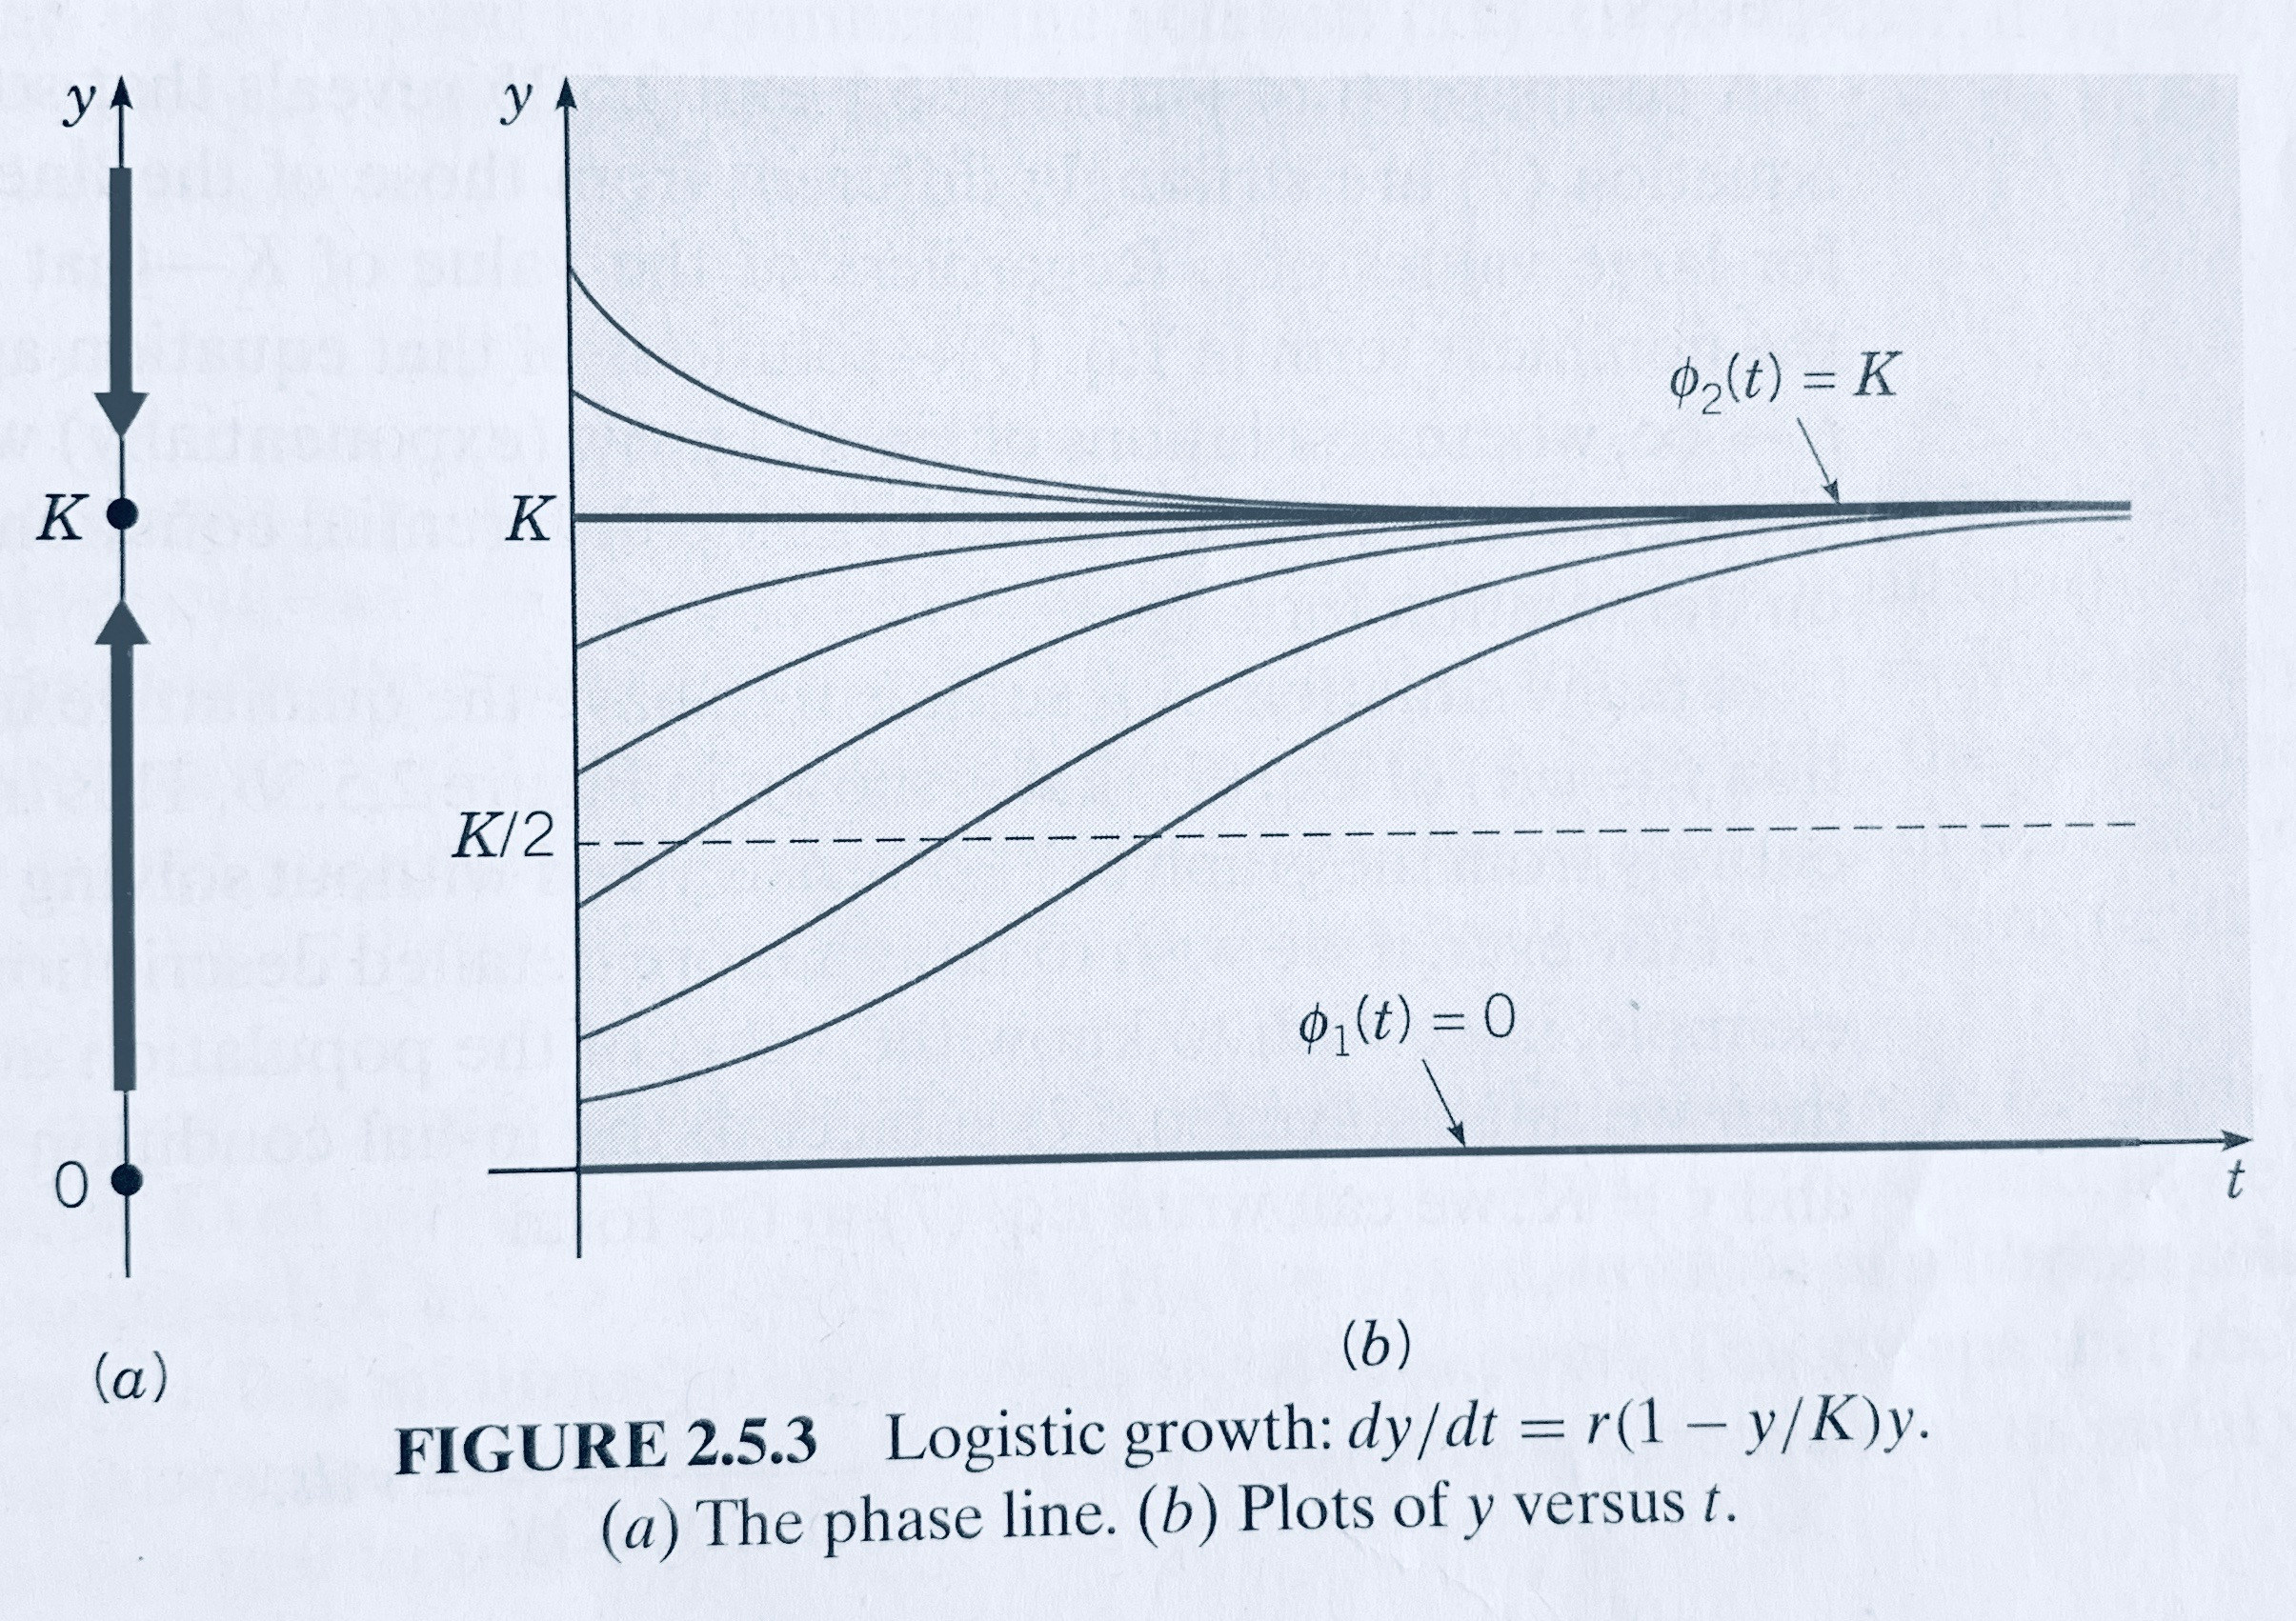
\includegraphics[width=200pt]{logistic_solutions.jpg}
    \end{center}
    $K$ is often referred to as the \textbf{saturation level}, or the \textbf{environmental carrying capacity}, for a given species.
    \newline \indent
    Sometimes this qualitative knowledge of the solution is enough, but to solve it, we can rewrite the equation as
    \begin{equation*}
        \frac{dy}{(1 - y/K)y} = r \; dt
    \end{equation*}
    where $y \neq 0$ and $y \neq K$. Using a partial fraction expansion, we have
    \begin{equation*}
        (\frac{1}{y} + \frac{1/K}{1-y/K})dy = r \; dt
    \end{equation*}
    By integration,
    \begin{equation*}
        \ln |y| - \ln |1 - \frac{y}{K}| = rt + c
    \end{equation*}
    since if $0 < y_0 < K$ then $y$ will remain in this interval, we can remove the absolute values. Then by taking the exponential of both sides,
    \begin{equation*}
        \frac{y}{1-(y/K)} = Ce^{rt}
    \end{equation*}
    where $C = e^c$. $C = y_0/[1-(y_0/K)]$ to satisfy $y(0) = y_0$.
    \begin{equation*}
        y = \frac{y_0K}{y_0 + (K - y_0)e^{-rt}}
    \end{equation*}
    We notice that 
    \begin{equation*}
        \lim_{t \rightarrow \infty} y(t) = K
    \end{equation*}
    hence $y = K$ is an \textbf{asymptotically stable solution}, and $y = 0$ is an \textbf{unstable equilibrium solution}.
    \newline
    \textbf{A Critical Threshold}. Consider the equation
    \begin{equation*}
        \frac{dy}{dt} = -r(1 - \frac{y}{T})y
    \end{equation*}
    The function $dy/dt = f(y)$ is a parabola with zeros at $y = 0$ and $y = K$ opening up. For $0 < y < T$, $f(y) < 0$. Hence $T$ is the \textbf{threshold level} since no growth occurs below it. Above $T$, $y$ grows indefinitely. It becomes unbounded in a finite amount of time $t*$.
    \begin{equation*}
        t* = \frac{1}{r}\ln\frac{y_0}{y_0 - T}
    \end{equation*}
    which we find by setting the denominator of the solution to 0.
    \newline
    \textbf{Logistic Growth with a Threshold.} This equation can be modified so that unbounded growth does not occur when $y$ is above $T$. We need another factor that makes $dy/dt$ negative when $y$ is large.
    \begin{equation*}
        \frac{dy}{dt} = -r(1 - \frac{y}{T})(1 - \frac{y}{K})y
    \end{equation*}
    This pulls $dy/dt$ back down after a certain point. $f(y)$ is a cubic function now. The solutions of the equation are similar to the equations with unbounded growth except when $y > T$, $y$ will approach $K$.
